% RoboSketch-RL - IEEE conference paper draft
% v1 2026-10-19 (skeleton, kept as main.tex.bak_2026-10-19); v2 2026-11-08 full draft from logged results, by Claude Code.
%
% RULES (enforced by check_paper.py - run it after every edit):
%  - every decimal number carries a "% src:" comment (this line or the next two) naming the
%    RESEARCH_LOG entry or file it came from
%  - \cite only keys that exist in references.bib (generated by make_bib.py - never hand-edit)
%  - wording no stronger than docs/PAPER_PLAN.md section 2
%  - compile LOCALLY only (MiKTeX / TeX Live). Do NOT upload to Overleaf or any website:
%    AGENTS.md section 2 - this is unpublished, confidential research.
%
% STATUS (2026-11-08): all sections drafted. Left open (\TODO): authors,
% acknowledgment / AI-use disclosure, a page-budget pass. Quotes verified vs PDFs 2026-11-08.
\documentclass[conference]{IEEEtran}
\usepackage{graphicx}
\usepackage{booktabs}
\usepackage{amsmath}
\usepackage{xcolor}
\newcommand{\TODO}[1]{\textcolor{red}{[TODO: #1]}}

\begin{document}

\title{What Does a Drawing Robot Lose by Learning from Its Camera?}
\author{Viral Kanani\\Independent researcher \TODO{email; confirm affiliation line}}
\maketitle

\begin{abstract}
Reinforcement-learning drawing agents are trained and rewarded on an exact virtual canvas,
a signal no physical robot has. We measure, in simulation, what changes when a pen-drawing
agent learns from what a simulated camera sees instead. On four simple shapes, policies
trained from a camera reward and from the privileged canvas reach true accuracy that is
statistically equivalent within 0.05 IoU (TOST, pre-registered margin); % src: RESEARCH_LOG "H2 spaced RESULT"
the camera reward is not exploited, and a fixed-camera policy loses little on a held-out
camera that recovers under half of the ink. A camera-free agent that tracks its drawing
through forward kinematics, as argued for by prior work, cannot see the sheet move. In a
pre-registered, replicated test, an agent that estimates the sheet offset from its own
photograph loses less to a paper shift than the kinematics agent in all 16 (shape, seed)
pairs. % src: RESEARCH_LOG "H4 v4 confirmation RESULT" (pooled 16/16)
It gains nothing detectable on pen slip or ink failure, and the estimator costs some
robustness there. We also report what limits the absolute level: agents finish early and
overshoot, generalise poorly to resized or rotated shapes unless the observation is
pen-centred, and sit far below a scripted tracer.
\end{abstract}

% ============================================================================
\section{Introduction}
Reinforcement-learning agents that draw and paint are trained against an exact virtual
canvas \cite{D02,D05,D06,D07,D01}. At every step the agent is rewarded by comparing a
perfect rendering of its own strokes with the target image. A physical robot has no such
canvas: the only record of what it has drawn is what a camera can see, through blur,
uneven lighting, imperfect registration and noise.

One response is to avoid the camera altogether. Lee et al.~\cite{D01} train a robotic
sketching agent that keeps its virtual canvas synchronised with the pen position the arm
actually reaches, i.e.\ through the robot's own kinematic state, so it assumes that
wherever the pen tip went, the mark appeared in the expected place on the sheet; they
attribute their agent's robustness to this camera-free design. % src: D01 PDF p.4 (Sec. III-D Stroker), p.6 (Sec. IV-B)
If that holds, there is little reason to put a camera in the learning loop at
all. The same authors nevertheless note that ``using a camera as an observation of canvas
in the future work could be of great help in the synchronization step''~\cite{D01}.
Kotani and Tellex point to ``closing the learning loop by enabling the robot to inspect
what it has drawn''~\cite{D03}, and Luo et al.\ leave ``a lack of real-world training
scenarios to bridge the sim2real gap'' as future work~\cite{D09}.
% quotes VERIFIED verbatim against the PDFs 2026-11-08: D01 p.6 (Sec. V), D03 p.6 (Sec. V), D09 p.6 (Sec. V)

This paper does not propose a new drawing algorithm. It \emph{measures} two things that
the closest prior work leaves open: how much drawing accuracy is lost when the agent
learns from what a simulated camera perceives instead of from the true canvas, and
whether seeing the paper lets the agent recover from errors that forward kinematics
cannot detect. Our contributions are:
\begin{itemize}
\item A pre-registered comparison of camera and privileged rewards: on four shapes the
  two are statistically equivalent in true accuracy within a 0.05 IoU margin (TOST), % src: RESEARCH_LOG "H2 spaced RESULT"
  and the camera reward is not exploited (Secs.~\ref{sec:h2},~\ref{sec:h3}).
\item Evidence that this survives a much worse camera, and that camera randomisation
  during training adds nothing detectable (Sec.~\ref{sec:dr}).
\item A replicated measurement against the camera-free position: for a disturbance that
  kinematics cannot see (the sheet sliding under the pen), an agent that estimates the
  sheet offset from its photograph loses less accuracy than a kinematics-synchronised
  agent; for pen slip and ink failure we detect no advantage (Sec.~\ref{sec:h4}).
\item Measurements that bound the absolute level and should inform how drawing agents are
  evaluated: early completion and overshoot, poor transfer to resized or rotated targets
  except with a pen-centred observation, and the gap to a scripted tracer
  (Secs.~\ref{sec:overrun},~\ref{sec:gen}).
\end{itemize}

% ============================================================================
\section{Related Work}
\textbf{Learning to draw.} Most learned drawing agents are trained against a rendered
canvas. Huang et al.~\cite{D02} learn a differentiable neural renderer and reward strokes
with a discriminator; SPIRAL~\cite{D05,D06} trains an agent with an adversarial reward
over a non-differentiable renderer; Zhou et al.~\cite{D07} combine deep Q-learning with
demonstrated strokes. CalliRewrite~\cite{D09} recovers stroke order without supervision
and then uses reinforcement learning to fine-tune that stroke sequence into control of a
simulated brush. In all of these the
reward is computed from an exact digital canvas. Kotani and Tellex~\cite{D03} infer a
continuous drawing plan from an image with supervised learning rather than reinforcement
learning. The robotic sketching agent of Lee et al.~\cite{D01} is the closest to ours and
the position this paper tests: it learns a decoupled stroke policy and motor policy and
deliberately operates without a camera. Ergodic control has been used to render images
with physical motion without learning~\cite{D04}; we use it as a non-learning comparator.
% Related Work paraphrases CHECKED vs PDFs 2026-11-08: D02 p.3 Eq.(1) (reward = discriminator score), D05 p.1, D06 p.1, D07 p.1, D09 p.1 (RL/SAC fine-tunes the coarse sequence into brush control), D03 p.1, D01 p.1, D04 p.1, R01 p.1, R02 p.1, A01 p.1, V01 p.1, V02 p.1

\textbf{Perceptual and learned rewards.} Rewarding a robot from images rather than from
privileged state is established in manipulation. Sermanet et al.~\cite{R01} build a dense
perceptual reward from pretrained visual features and a few demonstrations; Singh et
al.~\cite{R02} learn a reward classifier over raw images and train end to end on a real
robot. We do not claim image-based rewards as new; we measure what such a reward costs
for drawing specifically, where the reward is the drawing itself.

\textbf{Visual feedback in robot painting.} FRIDA~\cite{A01} photographs real strokes and
fits a differentiable painting simulator to them (real2sim2real), replanning against the
camera. Closed optical-feedback loops in robot painting go back at least to the
e-David machine~\cite{A09}, which photographs the canvas and places new strokes from the
difference to the target. These systems close the loop
at planning time; our question is what happens when the learning signal comes from the
camera.

\textbf{Domain randomisation.} Randomising simulated visual parameters so that the real
world looks like one more sample is a standard route to sim-to-real transfer~\cite{V01};
dynamics randomisation plays the same role for physical parameters~\cite{V02}. We use
camera randomisation as a stress test of the perception-reward result (Sec.~\ref{sec:dr}).

% ============================================================================
\section{Setup}
\label{sec:setup}
\textbf{Environment.} A pen moves over a square sheet of paper in a PyBullet simulation of
a KUKA arm, wrapped as a Gymnasium environment. The agent acts in pen space:
each action is a displacement $(\Delta x, \Delta y)$ and a pen-down flag, so the policy is
independent of the arm. In all experiments the pen point is moved directly (the arm-driven
mode exists and is used for validation only) and, except in Sec.~\ref{sec:ext}, the pen is
always down. The canvas is rendered at $128\times128$ pixels and the observation at
$64\times64$. Episodes last 240 steps of 0.014~m (60 steps in Sec.~\ref{sec:h4}). % src: rl/experiment.py --max-steps/--step-size defaults; results/h2_spaced_*.jsonl rows; rl/h4_short_experiment.py --max-steps 60
Targets are a line, a circle, a square and a triangle; the pen starts on the target, at
the point nearest the centre of the sheet.

\textbf{Observation.} A stack of image channels: the target, what has been drawn, and the
pen position. Where the drawn channel comes from is the experimental variable for H4:
\emph{true} (the real canvas, privileged), \emph{fk} (what forward kinematics predicts was
drawn, as in~\cite{D01}) or \emph{camera} (a simulated photograph).

\textbf{Reward.} Dense shaping toward higher intersection-over-union (IoU) with the target:
newly covered target pixels are rewarded, ink off the target is penalised, with a small
smoothness cost. In \emph{truth} mode the IoU is computed from the true canvas; in
\emph{vision} mode it is computed from the simulated camera image.

\textbf{Camera model.} The camera renders the sheet through an imaging chain of paper tone,
ink contrast, perspective warp, sensor resolution, blur, gain, noise and a binarisation
threshold. A single fixed setting is used unless stated; Sec.~\ref{sec:dr} samples these
parameters from a training distribution and evaluates on a disjoint held-out one.

\textbf{Learning and scoring.} All agents are trained with PPO~\cite{F01} (CNN policy,
8 parallel environments, 512 steps per rollout, batch 256, 6 epochs, $\gamma=0.99$,
entropy coefficient 0.02, learning rate $3\times10^{-4}$) for $2\times10^5$ steps. % src: rl/experiment.py PPO(...) / rl/h4_experiment.py PPO(...)
\textbf{Every reported score is the true IoU of the real canvas}, whatever the agent
observed or was rewarded with, so no agent is credited for what its camera believes.
Comparisons are paired within (shape, seed); we report the mean difference, the number
of pairs favouring each arm, and a one-sample $t$ statistic ($n=8$ pairs: critical
$|t| = 2.37$ at $p<0.05$, two-sided). Because PPO seeds its parallel environments % src: RESEARCH_LOG fix F6; t(7) critical value used by every --aggregate
consecutively, we use spaced seeds (0, 100, 200, 300); the overshoot ablation
(Sec.~
ef{sec:overrun}) predates this and used adjacent seeds 0 and 1. Main analyses were fixed in the research
log before the runs.

% ============================================================================
\section{Experiments}

\subsection{Does a camera reward cost drawing accuracy?}
\label{sec:h2}
We trained each shape with the truth reward and with the vision reward on three spaced
seeds (100, 200, 300; $n=12$ pairs) and tested equivalence with a margin of $\pm0.05$ IoU
fixed before the runs. Camera-rewarded policies reached a mean true IoU of
0.384 $\pm$ 0.059, against 0.388 $\pm$ 0.062 for the privileged reward % src: RESEARCH_LOG "H2 spaced RESULT"
(difference +0.004, privileged ahead in 6 of 12 pairs, $t=+0.27$; 90\% CI $[-0.024, +0.033]$). % src: RESEARCH_LOG "H2 spaced RESULT"
The two rewards are equivalent within the margin (TOST $p=0.008$), and also on peak IoU. % src: RESEARCH_LOG "H2 spaced RESULT"
The per-shape differences are not: the square favours the privileged reward by more than
the margin and the line and circle favour the camera, at $n=3$ per shape. An earlier sweep
on adjacent seeds (0, 1, 2), whose parallel environments overlap, gave a larger gap of
+0.028 whose CI $[-0.007, +0.063]$ does not pass the same test; % src: RESEARCH_LOG "H2 spaced RESULT" (contrast)
we report the pre-registered spaced-seed sweep and do not pool the two.

\begin{figure}[t]
\centering
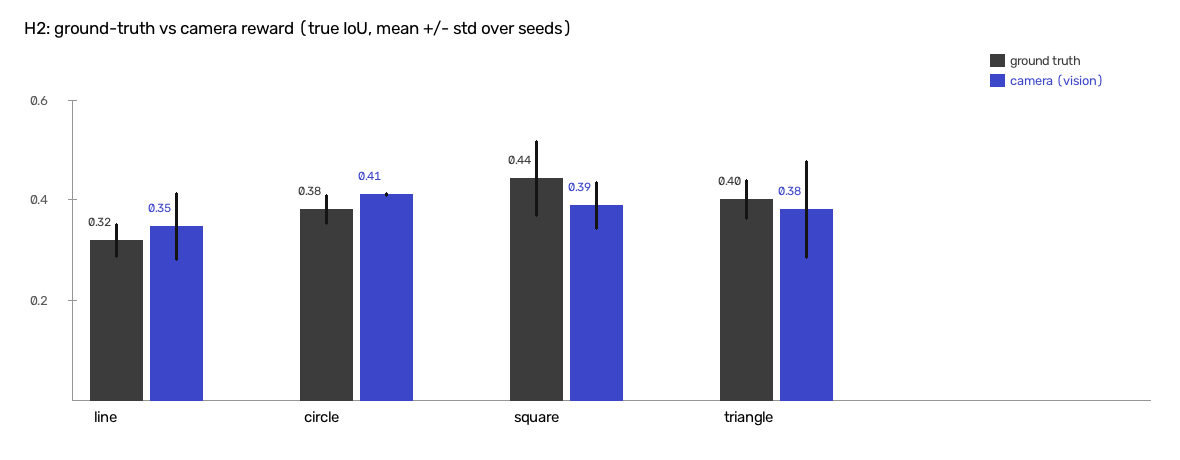
\includegraphics[width=\columnwidth]{../../output/results_h2_spaced.png}
\caption{True IoU of policies trained from the privileged canvas (truth) and from the
simulated camera (vision), spaced seeds 100/200/300. Scored on the real canvas.}
\label{fig:h2}
\end{figure}

\subsection{Is the camera reward exploited?}
\label{sec:h3}
An agent optimising a perceived score could learn to please the camera rather than to
draw. Logging both scores for every training episode, perceived minus true IoU averaged
$-0.0001$ over 3328 episodes, and the two correlated at 0.997--0.999 throughout training. % src: RESEARCH_LOG "H3 RESULT"
The residual has no consistent sign across shapes, and the truth-reward control shows a gap
of exactly zero. We see no evidence of reward exploitation (one seed per shape, fixed camera).

\subsection{Does it survive a worse camera?}
\label{sec:dr}
We trained three arms - the truth control, the fixed camera, and cameras resampled each
episode from a training distribution - and scored each under the fixed camera, a training
camera and a held-out camera outside the training distribution on every axis. The
held-out camera recovers only 0.394 of the ink in a perfect drawing, against 0.834 for % src: RESEARCH_LOG "Calibration, measured rather than asserted"
the fixed camera. Even so, the fixed-camera agent lost only 0.014 true IoU on it. % src: RESEARCH_LOG "STAGE 2 RESULT" + "Correction (2026-10-19)"
Training across randomised cameras did not improve on this: on the held-out camera the
randomised arm trailed the fixed arm by 0.011 ($t = -0.67$, $n = 8$). % src: RESEARCH_LOG "STAGE 2 RESULT"
The policy appears to need only a coarse record of where it has already drawn, which even
a poor camera preserves. Of the eight camera parameters, three (resolution, blur, residual
warp) carry the degradation; exposure, paper tone and ink contrast cancel by construction
because the threshold is set relative to the observed ink and paper levels. Absolute IoU
here is not comparable with Sec.~\ref{sec:h2}, because the camera is also in the observation.

\subsection{Does seeing the paper help recovery?}
\label{sec:h4}
\textbf{Design.} Three disturbances fire once during drawing and are applied to reality
only: \emph{slip} (the pen is knocked sideways), \emph{paper shift} (the sheet, with its
ink, slides under the pen) and \emph{ink failure} (the pen stops inking for a stretch).
Learning arms are trained on a random mix of disturbances and scored on each kind. The
\emph{fk} arm follows~\cite{D01}: its drawn channel is what kinematics predicts. A
camera-free agent cannot see a paper shift at all. The test statistic is the paired
difference-in-differences: how much \emph{less} an arm loses relative to its own
undisturbed score, so that an arm that simply draws better is not credited with recovery.
The \emph{fk} arm is rewarded from the true canvas and the camera arms from the camera,
an asymmetry that favours \emph{fk}.

\textbf{An exploratory series.} The first two designs (240- and 60-step episodes) were null:
the camera arm recovered no better than \emph{fk} on any disturbance ($|t| \le 1.19$ and % src: RESEARCH_LOG "H4 RESULT" + "H4-SHORT RESULT"
$|t| \le 0.79$), and neither did a privileged arm that sees the real canvas. With the % src: RESEARCH_LOG "H4-SHORT RESULT"
pen-position marker drawn in world coordinates, an agent that sees the shifted ink still
does not know where its pen is relative to the sheet. Drawing the marker in sheet
coordinates, using the simulator's true offset, removed most of the paper-shift loss for
camera and privileged arms alike (H4 v3); that is not a camera result, because the offset
was given. In the fourth design (v4) the camera arm \emph{estimates} the offset itself, by
phase correlation between the photograph and the canvas its kinematics expect, and draws
the marker accordingly (\emph{camera\_est}). The analysis and a replication on fresh seeds
were fixed in advance.

\textbf{Result.} Table~\ref{tab:h4} and Fig.~\ref{fig:h4} give the replication. On paper shift the
kinematics arm loses 0.165 IoU and the estimating camera arm 0.046: a difference-in-differences % src: RESEARCH_LOG "H4 v4 confirmation RESULT"
of $+0.119$, in favour of the camera in 8 of 8 pairs ($t=+8.32$). The two arms start level % src: RESEARCH_LOG "H4 v4 confirmation RESULT"
without disturbance ($+0.006$, $t=+0.37$), so this is a smaller loss, not a head start. % src: RESEARCH_LOG "H4 v4 confirmation RESULT"
The original seeds gave $+0.077$ (8/8, $t=+6.39$); over all 16 pairs the camera arm % src: RESEARCH_LOG "H4 v4 RESULT"
lost less in 16 of 16 ($+0.098$, $t=+9.32$). The estimate does not reach the true offset: % src: RESEARCH_LOG "H4 v4 confirmation RESULT" (pooled)
the arm given the simulator's offset loses 0.016, and \emph{camera\_est} loses 0.030 more % src: RESEARCH_LOG "H4 v4 confirmation RESULT"
($t=-2.42$, just past the critical value). For slip and ink failure we find no detectable difference % src: RESEARCH_LOG "H4 v4 confirmation RESULT"
from \emph{fk} ($+0.004$ and $+0.003$, $|t| \le 0.37$). Against a camera arm with the % src: RESEARCH_LOG "H4 v4 confirmation RESULT"
plain world-frame marker, however, the estimator costs robustness: \emph{camera\_est} loses
more to ink failure ($-0.036$, $t=-5.29$) and slip ($-0.021$, $t=-2.64$). A plausible but % src: RESEARCH_LOG "H4 v4 confirmation RESULT"
untested cause is that missing or displaced ink misleads the phase correlation.

\begin{table}[t]
\caption{H4 replication (seeds 200/300, $n=8$ pairs, 60-step episodes). True IoU without
disturbance (clean) and IoU lost to each disturbance (slip, paper shift, ink failure). Diff-in-diff vs \emph{fk}: $>0$ means the
arm loses less.}
\label{tab:h4}
\centering
\small
\setlength{\tabcolsep}{3pt}
\begin{tabular}{lcccc}
\toprule
arm & clean & slip & shift & ink \\
\midrule
open-loop tracer & 0.485 & 0.264 & 0.300 & 0.015 \\ % src: RESEARCH_LOG "H4 v4 confirmation RESULT"
fk (kinematics) & 0.369 & 0.008 & 0.165 & 0.045 \\ % src: RESEARCH_LOG "H4 v4 confirmation RESULT"
camera (world) & 0.358 & $-0.017$ & 0.108 & 0.005 \\ % src: RESEARCH_LOG "H4 v4 confirmation RESULT"
camera\_est & 0.375 & 0.004 & 0.046 & 0.041 \\ % src: RESEARCH_LOG "H4 v4 confirmation RESULT"
camera, true offset & 0.423 & 0.006 & 0.016 & 0.037 \\ % src: RESEARCH_LOG "H4 v4 confirmation RESULT"
\midrule
camera\_est $-$ fk (DiD) & & $+0.004$ & $+0.119$ & $+0.003$ \\ % src: RESEARCH_LOG "H4 v4 confirmation RESULT"
\quad pairs up, $t$ & & 4/8, 0.37 & 8/8, 8.32 & 5/8, 0.32 \\ % src: RESEARCH_LOG "H4 v4 confirmation RESULT"
\bottomrule
\end{tabular}
\end{table}

\begin{figure*}[t]
\centering
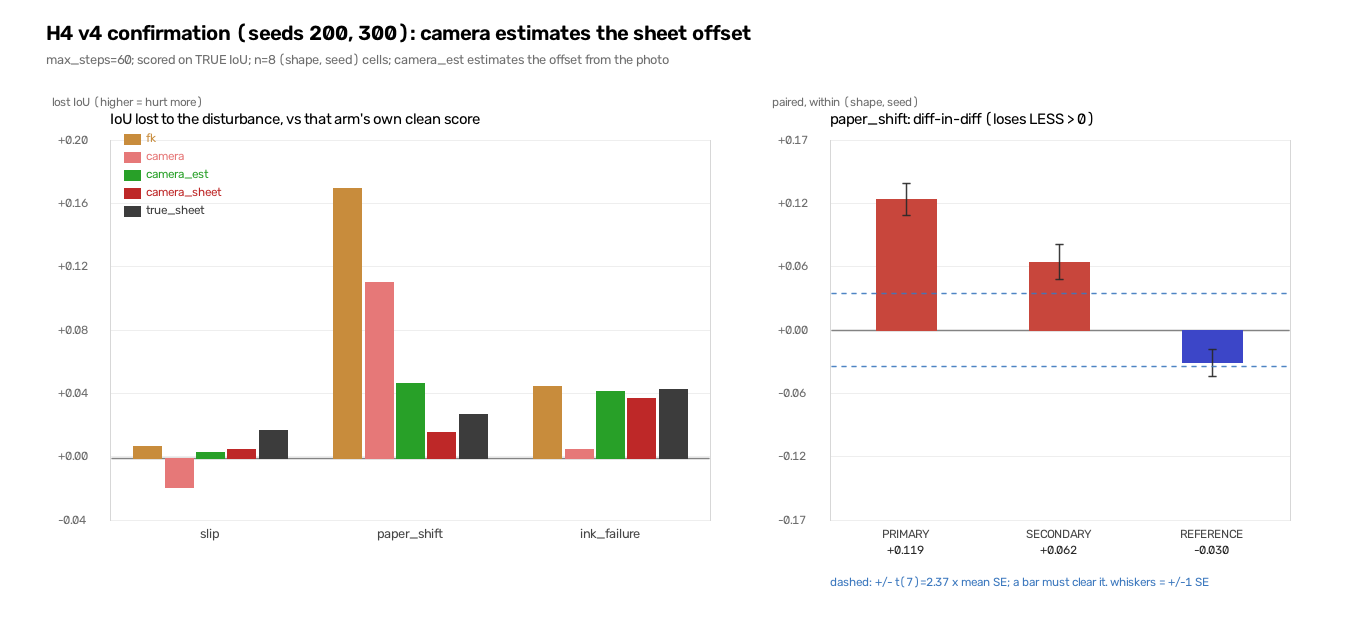
\includegraphics[width=\textwidth]{../../output/h4_confirm_recovery_seeds200_300.png}
\caption{H4 replication (seeds 200/300, $n=8$ (shape, seed) cells). Left: IoU each arm loses to each
disturbance, relative to its own clean score. \emph{camera\_sheet} is the camera arm given the true
sheet offset. Right: paired paper-shift diff-in-diff of \emph{camera\_est} against \emph{fk} (primary),
plain \emph{camera} and \emph{camera\_sheet}; a bar must clear the dashed line ($t_{7}$ critical value
times mean SE) to be detectable. Whiskers: $\pm 1$ SE.}
\label{fig:h4}
\end{figure*}

Ink failure barely bites in this setup (the open-loop tracer loses 0.015), so it cannot % src: RESEARCH_LOG "H4 v4 confirmation RESULT"
discriminate between arms. The result therefore supports the camera in the loop for one
disturbance kinematics is blind to, in simulation, with an estimator designed knowing that
the shift is a pure translation.

\subsection{Agents finish early and overshoot}
\label{sec:overrun}
Recording true IoU at every step, agents trace the shape within the first 10--17\% of the
episode (best IoU at step 12--41 of 240), overshoot briefly, and then leave the canvas % src: RESEARCH_LOG "UNEXPECTED FINDING - agents finish early"
unchanged for on average 74\% of the episode; the overshoot costs 0.064 IoU on average, % src: RESEARCH_LOG "UNEXPECTED FINDING - agents finish early"
more than twice the reward gap of the earlier H2 sweep. Ending episodes once IoU stops
improving raised true IoU from 0.378 to 0.433, but a plain 50-step horizon without any % src: RESEARCH_LOG "OVERSHOOT ABLATION RESULT"
stopping rule is not distinguishable from it ($+0.016$, $t=+0.63$) and gives most of the % src: RESEARCH_LOG "C5 4th arm RESULT"
gain ($+0.039$, $t=+1.59$, below the critical value at $n=8$). We present this as an evaluation % src: RESEARCH_LOG "C5 4th arm RESULT"
pitfall: final-step IoU understates what agents reach, and episode length matters; we
do not claim adaptive stopping as a fix. Reporting peak instead of final IoU did not change
the H2 comparison.

\subsection{Generalisation and the absolute level}
\label{sec:gen}
All results above use one fixed picture per shape. On targets resized and rotated beyond
the training range, fixed-target agents reach 0.074 true IoU; training on a family of % src: RESEARCH_LOG "Generalisation RESULT"
sizes and rotations raises this to 0.118 ($+0.044$, 8/8, $t=+7.35$), still far below the % src: RESEARCH_LOG "Generalisation RESULT"
home score. Three times more training ($+0.013$, $t=+0.95$) and coordinate channels % src: RESEARCH_LOG "Generalisation part 2 RESULT"
(CoordConv; $+0.008$, $t=+0.97$) did not help. A pen-centred 64-pixel observation did: % src: RESEARCH_LOG "O3 CoordConv RESULT"
held-out IoU rose from 0.118 to 0.298 ($+0.181$, 8/8, $t=+7.00$), not explained by the % src: RESEARCH_LOG "O2 egocentric RESULT"
extra pixel density alone (pen-centred minus a zoomed global view: $+0.161$, $t=+8.04$), % src: RESEARCH_LOG "O2z zoom control RESULT"
and surviving a camera in the loop (0.273 vs 0.130, $t=+3.54$). % src: RESEARCH_LOG "O2c RESULT"

The absolute level stays low. A scripted outline tracer that reads the target's parameters
reaches 0.72--0.74 true IoU on every target set, and a non-learning ergodic controller~\cite{D04} % src: RESEARCH_LOG "T1 BC warm start RESULT" (expert row)
that reads the target mask reaches about 0.30 on every set (held-out 0.306), level with % src: RESEARCH_LOG "Ergodic baseline RESULT"
the pen-centred agent and far above the global-view agent off-distribution. A policy cloned
from the tracer scored 0.591 on training targets before reinforcement learning, which then % src: RESEARCH_LOG "T1 BC warm start RESULT"
lowered it to 0.292. Our claims concern the gap between reward sources, not drawing quality. % src: RESEARCH_LOG "T1 BC warm start RESULT"

\subsection{Extensions: curriculum, pen lifting and digits}
\label{sec:ext}
Pre-training on the line before a target shape made the final result worse than training
from scratch (0.246 vs 0.418; $-0.173$, 5/6 pairs worse, $t=-2.99$, $n=6$). Letting the % src: RESEARCH_LOG "RQ4 curriculum RESULT"
agent control the pen on single-stroke shapes slowed learning and gave no detectable
change in final IoU (0.329 vs 0.418, $t=-2.29$, $n=6$). On digits, an exploratory run % src: RESEARCH_LOG "A2 pen-free RESULT"
found similar IoU for one- and two-stroke digits (0.309 vs 0.293) while an in-house % src: RESEARCH_LOG "Stage 6 digits RESULT"
recogniser read 3 of 4 one-stroke and 0 of 4 two-stroke drawings as the right digit
($n=4$ per group, no test), a reason to report legibility next to IoU for glyphs.

% ============================================================================
\section{Discussion and Limitations}
\textbf{What this means for camera-free drawing.} The camera-free argument of~\cite{D01}
rests on kinematic synchronisation being enough. In our simulation it is enough when the
world behaves: the camera reward costs no measurable accuracy, but it also buys nothing on
pen slip or ink failure. It is not enough when the sheet moves, which kinematics cannot
observe; there, a camera arm that estimates the sheet pose lost less in every pair over
four seeds. The benefit came only after the agent was told where its pen is \emph{on the
sheet}: two designs that gave the camera the image alone were null. Seeing the paper is
useful when the observation makes the paper's motion actionable.

\textbf{Limitations.} All results are in simulation, with a simulated camera bounded by the
eight parameters it varies, and four simple shapes; the H2 equivalence holds for fixed
pictures and pooled over shapes, not per shape. Seeds per configuration are two to three.
The H4 series was exploratory (two nulls, one privileged design) before the replicated
design; its paper shift is a pure translation seen by a near-fixed camera, and the
phase-correlation estimator was written knowing that. Ink failure barely bites and could
not discriminate. The \emph{fk} arm was rewarded from the true canvas. Agents generalise
poorly to new sizes and rotations unless the observation is pen-centred, and the absolute
IoU is far below a scripted tracer. Seeded results on this software stack also depend on
the thread count, so runs are compared only within one thread setting. No real robot or
real camera was used.

\section{Conclusion}
Learning to draw from a simulated camera instead of the privileged canvas cost no
measurable accuracy within 0.05 IoU (TOST) in our setting, and the camera reward was not % src: RESEARCH_LOG "H2 spaced RESULT"
exploited. Against a kinematics-only agent, a camera agent that estimates the sheet's
position lost less to a paper shift in a pre-registered replication, but showed no
detectable advantage for slip or ink failure. Testing this with a real camera and arm is
the next step.

\section*{Acknowledgment}
\TODO{guide / institution; and the venue's required disclosure of AI-assisted writing.}

\bibliographystyle{IEEEtran}
\bibliography{references}
\end{document}
